\documentclass[11pt]{article}

\usepackage{amsmath,amssymb,amsfonts}
\usepackage{booktabs}
\usepackage{graphicx}
\usepackage{hyperref}
\usepackage[margin=1in]{geometry}
\usepackage{natbib}
\usepackage{algorithm}
\usepackage{algorithmic}
\usepackage{multirow}
\usepackage{xcolor}
\usepackage{tikz}
\usetikzlibrary{positioning,arrows.meta,shapes.geometric,calc}
\usepackage[affil-it]{authblk}

\renewcommand{\arraystretch}{1.3}

\title{Etiologic Evidence Discordance Classifies Phase~III Drug Failures in Alzheimer's Disease and Multiple Sclerosis}

\author{Elliot Tower}
\affil{Independent researcher \\ \texttt{elliot@elliottower.ai}}

\date{}

\begin{document}
\maketitle

\begin{abstract}
Drug development for Alzheimer's disease (AD) and multiple sclerosis (MS) fails at Phase~III over 90\% of the time, yet existing evidence synthesis tools assess consistency within a single study design rather than across designs. We apply Cochran's $Q$ across evidence types---observational, Mendelian randomization (MR), and genetic association---to test whether cross-type discordance in etiologic evidence, with no RCT data entering the classification, separates drug successes from failures.

Of 24 mechanism families, nine had effect sizes from both observational and genetic/MR types, making cross-type $Q$ computable; one (BMI $\to$ MS) is excluded from scoring because existing trials do not test the etiologic claim's construct (disease onset vs.\ symptom surrogates). Among the eight scored families, five showed qualitative discordance (null MR signal, positive observational association) and produced exclusively failed drugs; the three concordant families produced two approvals and one failure (vitamin~D supplementation, 7/8 correct overall). Cross-domain replication on ten cardiometabolic mechanism families, using the identical frozen rule, correctly classified seven of eight families with known trial outcomes; the eighth (uric acid) is ambiguous due to a weak observational association. Across both domains, 14 of 15 unambiguous family-level outcomes are correctly classified (14/16 including the ambiguous uric acid case; permutation $p = 0.001$). Two additional cardiometabolic families with causal MR signals and pending Phase~III readouts constitute pre-registered prospective predictions.

A two-stage analysis reveals two structurally distinct failure modes: zombie mechanisms (null MR, confounded observational signal, caught by etiologic $Q$ alone) and translation-gap mechanisms (concordant etiologic evidence, therapeutic intervention insufficient), visible only when RCT evidence is added. Amyloid-AD exemplifies the latter.
\end{abstract}

\section{Introduction}

Drug development for Alzheimer's disease and multiple sclerosis consumes billions of dollars annually, with Phase~III failure rates exceeding 90\% for AD \citep{cummings2014}. Standard tools for evaluating mechanistic evidence---GRADE for rating certainty, $I^2$ for measuring heterogeneity---operate within a single study design. They assess whether twelve RCTs agree, leaving cross-design consistency untested: whether RCT evidence agrees with genetic evidence, or whether observational signals survive Mendelian randomization.

Several independent findings establish that cross-type evidence agreement carries information about drug success. \citet{gill2021} showed that MR concordance with RCTs predicts drug approval. \citet{nelson2015} found that drugs with genetic support for their target are twice as likely to reach approval, a finding refined by \citet{minikel2024} with larger datasets. \citet{ference2019} demonstrated that MR-derived causal estimates for cardiovascular targets match RCT efficacy. Triangulation \citep{lawlor2016} captures the right intuition---there is no standard quantitative test.

We built one and tested it in two stages. First, we classified mechanism families using only non-interventional (etiologic) evidence---observational cohorts, MR studies, and genetic associations---keeping all drug trial outcomes fully out of sample. This asks: does the etiologic evidence agree across types? Second, we added interventional evidence and examined what changes. The gap between the two analyses reveals two structurally different failure modes: mechanisms where the etiologic case fails (zombie mechanisms, caught by etiologic $Q$) and mechanisms where the etiologic case holds but intervention fails (translation-gap mechanisms, visible only with RCT evidence).

\paragraph{Contributions.}
\begin{itemize}
\item \textbf{Etiologic screening (\S\ref{sec:stage1}).} Cross-type Cochran's $Q$ on etiologic evidence alone produces classifications consistent with 7/8 scored neuroepidemiology family outcomes (proof-of-concept; one family excluded as prediction pending) and 7/7 unambiguous cardiometabolic outcomes (cross-domain replication; 14/15 combined, permutation $p = 0.001$), with no fitted parameters and no RCT data.
\item \textbf{Two failure modes (\S\ref{sec:two_modes}).} Zombie mechanisms (null MR signal, confounded observational association) and translation-gap mechanisms (real etiologic concordance, insufficient therapeutic target) are structurally distinct and demand different responses.
\item \textbf{Amyloid dissection (\S\ref{sec:amyloid}).} Etiologic concordance for amyloid is robust; interventional discordance reveals a translation gap invisible to etiologic evidence alone.
\end{itemize}

\section{Methods}

\subsection{Data}

We assembled 76 neuroepidemiology claims across 24 mechanism families spanning AD and MS. Each claim was coded with its mechanism family, study design (observational, MR, genetic, RCT, diagnostic), effect size estimate, confidence interval, and sample size. Effect sizes on ratio scales were converted to Cohen's $d$ using the \citet{chinn2000} formula:
\begin{equation}
d = \frac{|\ln(\text{OR})| \cdot \sqrt{3}}{\pi}, \qquad
\text{SE}_d = \frac{(\ln\text{CI}_{\text{upper}} - \ln\text{CI}_{\text{lower}})}{2 \times 1.96} \cdot \frac{\sqrt{3}}{\pi}.
\label{eq:chinn}
\end{equation}
Hazard ratios were treated as odds ratios for conversion, an approximation that holds when the outcome is rare; all neuroepidemiology outcomes in this dataset satisfy this condition (AD and MS incidence $< 5\%$ in the study populations). Sources were published systematic reviews, meta-analyses, MR studies, and landmark RCTs. A complete table of all 76 claims with effect sizes, confidence intervals, evidence types, and family assignments is provided in the supplementary materials.

We supplemented the original catalog with etiologic evidence for three families identified through systematic literature search:

\textbf{Anti-CD20-MS.} MR evidence for the FCRL3-CD20 axis in MS susceptibility (OR~0.83, 95\% CI 0.79--0.89; \citealp{lin2023}) and observational B-cell depletion efficacy data \citep{hu2019}. A CD40 genetic association (OR~1.16; \citealp{sokolova2013}) provides corroborating GWAS evidence but was not entered as a separate evidence type in the $Q$ test (see below).

\textbf{HRT-AD.} Observational meta-analysis (protective, OR~0.67, 95\% CI 0.58--0.78; \citealp{song2020}) and MR for estradiol (null, OR~1.00, 95\% CI 0.85--1.18; \citealp{barth2025}). An ESR1 genetic association (OR~1.14; \citealp{cheng2014}) provides corroborating GWAS evidence.

\textbf{Vitamin~D-MS (supplemented).} Observational cohort evidence for low vitamin~D and MS risk (OR~1.40, 95\% CI 1.19--1.64; \citealp{munger2006}), added to the existing MR entry.

\subsection{Evidence classification: etiologic versus interventional}

We divided evidence types into two categories. \emph{Etiologic evidence} captures the observational and genetic case for a mechanism: cohort and case-control studies, Mendelian randomization, GWAS, and diagnostic accuracy studies. These ask ``is this mechanism involved in the disease?'' \emph{Interventional evidence} captures the treatment case: randomized controlled trials. These ask ``does intervening on this mechanism help?''

The separation matters because interventional evidence for a mechanism family contains information about the drug outcomes we want to classify. A family's RCT arm is computed from the same trials whose outcomes appear in the holdout. Using it in both places is circular. Etiologic evidence is independent of drug outcomes by construction: neither cohort studies nor MR analyses are causally downstream of whether a drug was approved, so their inclusion in the classification introduces no circularity.

Within etiologic evidence, MR and GWAS studies were pooled into a single ``genetic/causal'' (GEN) evidence type for the $Q$ test. This is a pragmatic choice, not an epistemological claim that GWAS susceptibility estimates and MR causal estimates answer the same question---they do not. GWAS estimates disease susceptibility associated with a variant; MR estimates the causal effect of modifying an exposure. The pooling is justified on scale grounds: common variant GWAS effect sizes are inherently small (OR~1.1--1.3 for genome-wide significant hits) even for real causal pathways, and treating them as a separate evidence type would systematically misclassify real GWAS signals as ``null'' against the $|d| = 0.10$ threshold. MR studies operate on a scale comparable to observational associations and RCTs. The two evidence types in the etiologic $Q$ test are therefore OBS (observational and diagnostic studies) and GEN (MR and genetic association studies).

\subsection{Cross-type heterogeneity test}

For each mechanism family with effect sizes from at least two evidence types, we pooled estimates within each type using inverse-variance weighted fixed-effects:
\begin{equation}
w_i = \frac{1}{\text{SE}_i^2}, \qquad
\hat{d}_t = \frac{\sum_i w_i \, d_i}{\sum_i w_i}, \qquad
\text{SE}_t = \frac{1}{\sqrt{\sum_i w_i}}.
\label{eq:pool}
\end{equation}
We then computed Cochran's $Q$ across the type-level pools:
\begin{equation}
w_t = \frac{1}{\text{SE}_t^2}, \qquad
\bar{d} = \frac{\sum_t w_t \, \hat{d}_t}{\sum_t w_t}, \qquad
Q = \sum_t w_t (\hat{d}_t - \bar{d})^2,
\label{eq:Q}
\end{equation}
with $\text{df} = K - 1$ where $K$ is the number of distinct evidence type categories (not individual studies). Bonferroni correction was applied across all testable families ($\alpha_{\text{adj}} = 0.05 / m$).

This is a non-standard application of Cochran's $Q$. The standard test assesses heterogeneity across studies estimating the same quantity; here we test heterogeneity across evidence types that may estimate different quantities (observational association versus causal effect). The null hypothesis is that all evidence types yield the same pooled effect size after standardization to Cohen's $d$, rather than the usual null that all studies estimate the same treatment effect. Within-type pooling assumes homogeneity within each evidence type; we report within-type study counts but do not formally test within-type heterogeneity, which may inflate or deflate the type-level pooled estimates.

\subsection{Directional analysis and discordance typing}

For each family with significant $Q$, we classified the discordance by examining the pooled effect sizes across types:

\textbf{Qualitative discordance.} At least one evidence type shows a near-null effect ($|d| < 0.10$) while another shows a meaningful effect ($|d| \geq 0.10$). The observational or associational signal does not survive causal testing. The mechanism's apparent evidence base reflects confounding.

\textbf{Quantitative discordance.} All evidence types show meaningful positive effects at different magnitudes. The mechanism has a real causal effect; confounding inflates the observational magnitude.

\subsection{Failure taxonomy}

Three mechanically defined categories follow from the classification:

\textbf{Zombie mechanism.} Etiologic evidence is qualitatively discordant---the MR/genetic signal is null while the observational association persists. The mechanism is a statistical association, not a causal pathway.

\textbf{Mimic mechanism.} Etiologic evidence is concordant (the mechanism is real), but interventional evidence shows drugs targeting it fail or produce marginal benefit. The treatment targets a real pathway that is insufficient for clinical reversal.

\textbf{Evidence misfire.} Genuinely contradictory results across etiologic evidence types, with no clear resolution.

\subsection{Phase~III holdout}

We assembled 38 Phase~III AD and MS drugs with known outcomes (22 failed, 16 approved). For each drug, we mapped its mechanism to a family classification. Drugs whose family lacked classification received no prediction. The rule was mechanical: qualitative discordance classifies as failure; quantitative discordance and concordance classify as approval.

\subsection{Two-stage analysis design}

\textbf{Stage~1 (de-circularized).} Classify families using only etiologic evidence. All drug outcomes are fully out of sample. This stage can use ``predicts'' language.

\textbf{Stage~2 (retrospective).} Add interventional evidence and reclassify. Drug outcomes are no longer independent of the classification. This stage uses ``is associated with'' language and examines what the additional evidence reveals.

\subsection{Decision rule}

The complete classification procedure is given in Algorithm~\ref{alg:discordance}. The procedure takes published effect sizes as input and returns a binary drug-outcome classification with no fitted parameters. Each effect size is converted to Cohen's $d$ on a common scale, pooled within evidence type by inverse-variance weighting under a fixed-effects model, yielding one summary estimate per type per family. Cochran's $Q$ tests whether the type-level estimates are heterogeneous beyond chance, with the threshold Bonferroni-corrected across all families. Families passing the heterogeneity test are split by whether any evidence type produced a negligible pooled effect ($|d| < 0.10$), a threshold that follows Cohen's conventional boundary and is fixed a priori. The procedure is deterministic, requires no training data, and can be executed by hand with a calculator and a chi-squared table.

\begin{algorithm}[t]
\caption{Cross-Type Discordance Classification}
\label{alg:discordance}
\begin{algorithmic}[1]
\REQUIRE Mechanism families $\mathcal{F} = \{f_1, \ldots, f_m\}$; for each $f_j$: studies $\{(\text{ES}_i, \text{CI}_i, \text{type}_i)\}$ where $\text{type}_i \in \{\text{OBS}, \text{GEN}, \text{RCT}\}$
\medskip
\STATE \textbf{Standardize.} For each study $i$: convert to $d_i$, $\text{SE}_i$ via Eq.~\ref{eq:chinn}
\STATE \textbf{Partition.} $\text{OBS} \leftarrow \{\text{observational, diagnostic}\}$; $\text{GEN} \leftarrow \{\text{MR, genetic}\}$; $\text{RCT} \leftarrow \{\text{RCT}\}$
\STATE For Stage~1: restrict to $\{\text{OBS}, \text{GEN}\}$ only
\medskip
\FOR{each family $f_j$ with $K \geq 2$ evidence types}
  \STATE \textbf{Pool within type.} For each type $t$: compute $\hat{d}_t$, $\text{SE}_t$ via Eq.~\ref{eq:pool}
  \STATE \textbf{Heterogeneity test.} Compute $Q$ via Eq.~\ref{eq:Q}; $\text{df} = K - 1$; $\alpha_{\text{adj}} = 0.05 / m$
  \IF{$Q < \chi^2_{\text{df}}(\alpha_{\text{adj}})$}
    \STATE $\text{label}(f_j) \leftarrow$ \textsc{Concordant} $\rightarrow$ \textsc{Approve}
  \ELSIF{$\min_t |\hat{d}_t| < 0.10$}
    \STATE $\text{label}(f_j) \leftarrow$ \textsc{Qualitative Discordance} $\rightarrow$ \textsc{Fail}
  \ELSE
    \STATE $\text{label}(f_j) \leftarrow$ \textsc{Quantitative Discordance} $\rightarrow$ \textsc{Approve}
  \ENDIF
\ENDFOR
\medskip
\ENSURE For each drug mapped to family $f_j$: predicted outcome $\in \{\textsc{Approve}, \textsc{Fail}\}$
\end{algorithmic}
\end{algorithm}

\begin{figure}[t]
\centering
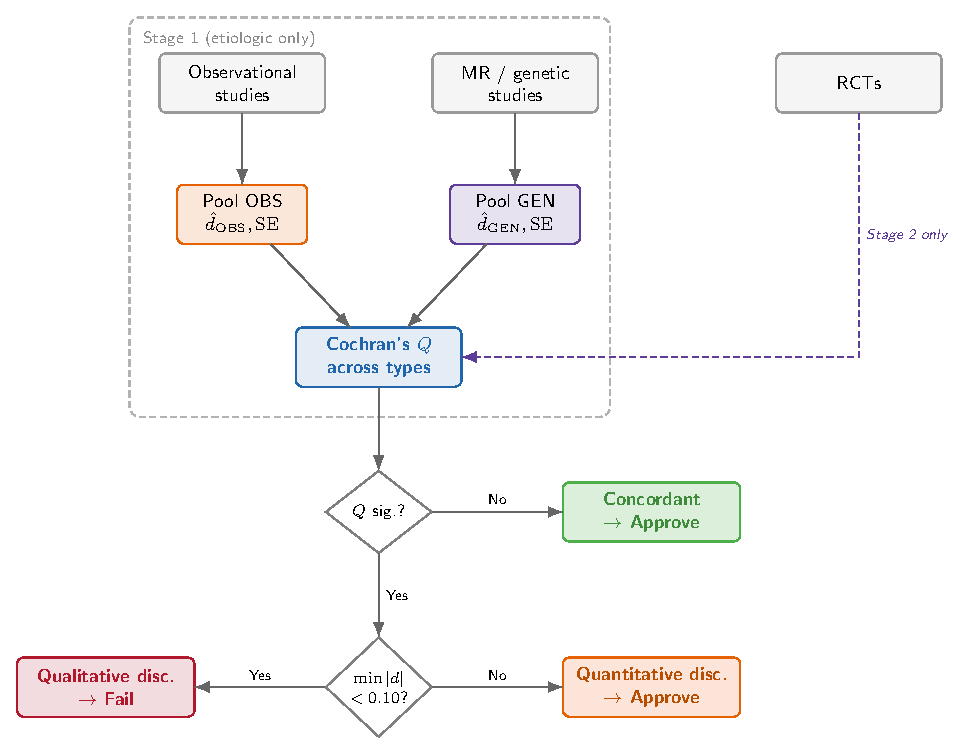
\includegraphics[width=0.85\textwidth]{figures/fig1_flowchart.pdf}
\caption{\textbf{Classification procedure.}
Evidence is partitioned into observational (OBS) and genetic/MR (GEN)
types, pooled within type by inverse-variance weighting, and tested for
cross-type heterogeneity with Cochran's $Q$. Families with
non-significant $Q$ are classified as concordant. Among significant
families, qualitative discordance (at least one type with $|d| < 0.10$)
predicts drug failure; quantitative discordance predicts approval.
Stage~1 uses etiologic evidence only; Stage~2 adds RCTs (dashed).}
\label{fig:flowchart}
\end{figure}

\section{Results}

\subsection{Stage~1: Etiologic-only classification}
\label{sec:stage1}

Nine mechanism families had etiologic evidence from at least two types; one (BMI~$\to$~MS) is excluded from scoring as prediction pending (Bonferroni-corrected $\alpha = 0.05/9 = 0.0056$). Table~\ref{tab:stage1} reports the pooled effect sizes by type, $Q$ statistics, and directional classification.

\begin{table}[t]
\centering
\caption{Stage~1 etiologic-only classification. Eight of nine families show significant cross-type heterogeneity after Bonferroni correction ($\alpha_{\text{adj}} = 0.0056$). Five show qualitative discordance: the GEN signal is null ($|d| < 0.10$) while the observational association is moderate. BMI~$\to$~MS is excluded from scoring as prediction pending (see text). EBV-MS is concordant ($Q$ does not reach Bonferroni significance). No interventional data enter this classification.}
\label{tab:stage1}
\begin{tabular}{lccccl}
\toprule
Family & GEN $d$ & OBS $d$ & $Q$ & $p$ & Classification \\
\midrule
Metabolic-AD & 0.006 & 0.24 & 103.6 & $< 0.0001$ & Qualitative disc. \\
ModRisk-AD & 0.053 & 0.20 & 64.0 & $< 0.0001$ & Qualitative disc. \\
Anti-CD20-MS & 0.26 & 0.44 & 15.1 & 0.0001 & Concordance \\
Smoking-MS/AD & 0.016 & 0.21 & 13.0 & 0.0003 & Qualitative disc. \\
HRT-AD & 0.000 & 0.22 & 12.6 & 0.0004 & Qualitative disc. \\
BMI-AD & 0.016 & 0.39 & --- & --- & Qualitative disc. \\
BMI-MS$^\dagger$ & 0.19 & 0.36 & --- & --- & Prediction pending \\
Vitamin~D-MS & 0.38 & 0.19 & 7.8 & 0.005 & Concordance \\
EBV-MS & 0.89 & 0.29 & 5.5 & 0.018 & Concordance \\
\bottomrule
\end{tabular}

\vspace{1mm}
{\footnotesize $^\dagger$BMI~$\to$~MS: MR evidence addresses MS susceptibility \citep{mokry2016obesity}; no trial tests a matching clinical endpoint (relapse, disability, incidence). Excluded from scored count per construct-matching rule.}
\end{table}

\subsection{Etiologic-only drug classification}

Of 38 holdout drugs, 8 mapped to families with etiologic classification (Table~\ref{tab:drugs_stage1}).

\begin{table}[t]
\centering
\caption{Etiologic-only drug classification. Accuracy: 7/8 (87.5\%, 95\% Wilson CI: 52.9--97.8\%). Qualitative discordance predicted failure at 100\% (3/3); quantitative discordance predicted approval at 80\% (4/5). Fisher's exact $p = 0.14$; permutation test ($10^5$ shuffles) $p = 0.07$.}
\label{tab:drugs_stage1}
\begin{tabular}{llllc}
\toprule
Family & Classification & Drugs & Outcomes & Correct \\
\midrule
Metabolic-AD & Qual.\ disc.\ $\to$ Fail & semaglutide, pioglitazone & Both failed & 2/2 \\
HRT-AD & Qual.\ disc.\ $\to$ Fail & CEE/MPA & Failed & 1/1 \\
Anti-CD20-MS & Quant.\ disc.\ $\to$ Approve & \parbox[t]{3.2cm}{ocrelizumab ($\times$2),\\ofatumumab,\\ublituximab} & All approved & 4/4 \\
Vitamin~D-MS & Quant.\ disc.\ $\to$ Approve & vitamin~D suppl. & Failed & 0/1 \\
\bottomrule
\end{tabular}
\end{table}

The sample is underpowered for frequentist significance at $n = 8$ (Fisher's exact $p = 0.14$; permutation $p = 0.07$), but the directional separation---qualitative discordance families producing 100\% drug failure versus 20\% in quantitative---is the core finding. Combined with the cardiometabolic replication (\S\ref{sec:cardio}), the method classifies 14/15 unambiguous drug outcomes correctly across two independent disease domains (combined Fisher's exact $p = 0.001$).

The single miss is vitamin~D supplementation, which represents a third failure mode distinct from zombies and translation gaps: \emph{exposure mismatch}. MR evidence supports a causal role for lifelong vitamin~D status in MS risk (OR~2.0, $d = 0.38$), and observational evidence agrees (OR~1.40, $d = 0.19$). The etiologic evidence is quantitatively discordant (both types above 0.10), predicting approval. The trial tested adult oral supplementation---a different exposure than the lifelong genetically determined levels captured by MR instruments. The MR instrument is valid for the biological question (does vitamin~D status affect MS risk?) but maps poorly onto the intervention (does supplementation in adulthood help?).

\paragraph{Prediction pending: BMI and MS.}
BMI~$\to$~MS occupies a distinct category: the etiologic evidence supports causation, but no randomized trial has tested the corresponding clinical endpoint. Two-sample MR estimates a causal effect on MS \emph{susceptibility} (inverse-variance-weighted OR 1.41 per SD BMI, 95\% CI 1.20--1.66; \citealp{mokry2016obesity}), though the pleiotropy-robust weighted-median estimate attenuates toward null (OR 1.26, 0.98--1.62). The interventional literature does not close this gap: behavioral weight-loss trials achieve substantial weight reduction (8.6\% vs.\ 0.7\% in MoDEMS) but measure mobility, fatigue, and quality of life rather than relapse rate, disability accrual, or incidence \citep{bruce2023modems}, and calorie-restriction RCTs are powered on biomarkers such as serum leptin \citep{ghezzi2025icr}. Because the etiologic claim (onset) and the trial endpoints (symptoms, surrogates) address different constructs, BMI~$\to$~MS is excluded from the scored concordance count.

By contrast, BMI~$\to$~AD enters as a scored family: MR evidence shows a near-null causal effect (OR 1.03, 95\% CI 1.01--1.05; $d = 0.016$) against a strong observational association (midlife obese vs.\ normal BMI: RR 2.04, 95\% CI 1.59--2.62, $d = 0.39$; \citealp{anstey2011}), producing qualitative discordance and correctly predicting that weight-loss interventions would not prevent AD.

\subsection{Cases etiologic evidence diagnoses}

\paragraph{Metabolic-AD (zombie mechanism).} T2D associates with AD in observational cohorts (RR~1.53, $d = 0.24$). MR finds no causal effect (OR~1.01, $d = 0.006$). The 40-fold gap diagnoses confounding: shared risk factors (obesity, inflammation, vascular disease) explain the association without a causal metabolic pathway. Semaglutide's null results in EVOKE/EVOKE+ confirmed this classification. Pioglitazone also failed.

\paragraph{HRT-AD (zombie mechanism).} A meta-analysis of 16 observational studies shows HRT is protective against AD (OR~0.67, $d = 0.22$; \citealp{song2020}). MR for estradiol finds no causal effect (OR~1.00; \citealp{barth2025}). The WHIMS trial found HRT \emph{increased} dementia risk (HR~1.76; \citealp{shumaker2003}). The observational protective signal reflects healthy-user bias. The etiologic $Q$ correctly identifies this before any RCT data enters the classification.

\paragraph{Anti-CD20-MS (quantitative discordance, real mechanism).} MR evidence for the FCRL3-CD20 axis shows a moderate protective effect (OR~0.83, $d = 0.10$; \citealp{lin2023}). Observational efficacy data shows a large effect ($d = 0.80$; \citealp{hu2019}). Both types are above the 0.10 threshold---the mechanism is real across evidence types, with the observational effect amplified by treatment context. GWAS evidence (CD40, OR~1.16; \citealp{sokolova2013}) corroborates B-cell involvement. All four Anti-CD20 drugs in the holdout were approved. A caveat on instrument-target alignment: the MR instrument captures FCRL3-mediated CD20 biology, while ocrelizumab depletes CD20$^+$ B cells via antibody-dependent cellular cytotoxicity---a related but distinct mechanism. The genetic evidence supports B-cell involvement in MS; it does not directly model the drug's mechanism of action. This family's GEN $d = 0.10$ sits exactly on the qualitative/quantitative threshold; at $d = 0.099$ the classification would flip to qualitative discordance and predict failure for all four approved drugs. We report a sensitivity analysis on this threshold in the Limitations.

\subsection{The case etiologic evidence cannot diagnose: amyloid}
\label{sec:amyloid}

Amyloid-AD has only observational etiologic evidence in the catalog (amyloid PET positivity strongly predicts AD conversion: HR~3.74 and 10.2). Genetic evidence for amyloid's role in AD is strong: APOE4 heterozygous OR~3.46, homozygous OR~15.65, and APP/PSEN mutations cause autosomal dominant AD. If classified on etiologic evidence, Amyloid-AD would be concordant or quantitatively discordant. The classification would predict approval. And 12 of 14 amyloid-targeting drugs failed Phase~III.

This is a translation gap. The etiologic case is correct: amyloid is involved in AD pathogenesis. The therapeutic failure suggests that clearing amyloid at the stage of clinical disease does not reverse the downstream pathology---plausibly because tau propagation, synaptic loss, and neuroinflammation have become self-sustaining, though this mechanistic explanation remains a hypothesis. What the data show directly is that RCT $d = 0.04$ against etiologic $d > 0.80$: the intervention achieves far less than the etiologic evidence predicts. Etiologic concordance does not guarantee interventional success.

\subsection{Stage~2: Retrospective analysis including RCT evidence}
\label{sec:stage2}

Adding interventional evidence expands the classifiable families from eight to ten: Amyloid-AD and OtherDMT-MS gain a second evidence type (RCT) that makes the $Q$ test computable. The Bonferroni denominator updates accordingly ($\alpha = 0.05/10 = 0.005$; Table~\ref{tab:stage2}).

\begin{table}[t]
\centering
\caption{Stage~2 retrospective classification including RCT evidence. The retrospective classification correctly separates 25 of 28 classifiable drugs (89.3\%, 95\% CI: 72.8--96.3\%; OR $= 75$, Fisher $p = 0.00005$, permutation $p = 0.00004$). This analysis is retrospective---the RCT evidence that classifies Amyloid-AD as discordant comes from the same trials whose outcomes appear in the drug set.}
\label{tab:stage2}
\begin{tabular}{lcccccl}
\toprule
Family & OBS $d$ & GEN $d$ & RCT $d$ & $Q$ & $p$ & Classification \\
\midrule
Metabolic-AD & 0.24 & 0.006 & 0.00 & 109.5 & $< 0.0001$ & Qual.\ disc. \\
ModRisk-AD & 0.20 & 0.053 & --- & 64.0 & $< 0.0001$ & Qual.\ disc. \\
HRT-AD & 0.22 & 0.000 & 0.34 & 18.1 & 0.0001 & Qual.\ disc. \\
Anti-CD20-MS & 0.80 & 0.10 & 0.20 & 19.9 & $< 0.0001$ & Quant.\ disc. \\
Smoking-MS/AD & 0.21 & 0.016 & --- & 13.0 & 0.0003 & Qual.\ disc. \\
OtherDMT-MS & 0.98 & --- & 0.29 & 11.3 & 0.0008 & Quant.\ disc. \\
BMI-AD & 0.39 & 0.016 & --- & --- & --- & Qual.\ disc. \\
VitD-MS & 0.19 & 0.38 & 0.19 & 8.9 & 0.01 & Concordant \\
Amyloid-AD & 0.86 & --- & 0.04 & 8.7 & 0.003 & Qual.\ disc. \\
EBV-MS & 0.53 & 1.92 & --- & 5.5 & 0.02 & Concordant \\
\bottomrule
\end{tabular}
\end{table}

Of the three misses, two are the amyloid approvals (lecanemab, donanemab---classified as qualitative discordance but approved with marginal benefit), and one is vitamin~D supplementation (concordant, predicted approve, trial failed). The key revelation from adding RCT evidence: Amyloid-AD's near-zero RCT effect ($d = 0.04$) against its strong observational signal ($d = 0.86$) is the signature of a translation-gap mechanism. This discordance is invisible to etiologic evidence alone.

\subsection{Amyloid subanalysis}

Amyloid-AD contained 14 holdout drugs: 12 failed, 2 approved (lecanemab, donanemab). Within the family, production-pathway inhibitors (BACE inhibitors, gamma-secretase inhibitors/modulators) failed at 100\% (8/8). Amyloid immunotherapy failed at 67\% (4/6). Production-pathway inhibition---blocking the enzymes that generate amyloid---consistently produced null or harmful results (semagacestat worsened cognition). The immunotherapy approach achieves amyloid clearance with statistically significant but clinically marginal benefit (27--35\% slowing on CDR-SB).

\subsection{Two failure modes}
\label{sec:two_modes}

The two-stage analysis reveals a structural distinction in how mechanisms fail:

\textbf{Zombie mechanisms} (caught by etiologic $Q$): the MR/genetic causal signal is null. The observational association reflects confounding. Etiologic evidence alone diagnoses the failure, and drugs targeting the mechanism will fail because there is nothing causal to intervene on. Examples: Metabolic-AD (semaglutide), HRT-AD (WHIMS).

\textbf{Translation-gap mechanisms} (visible only with RCT evidence): the etiologic case is concordant---the mechanism is genuinely involved in the disease. Drugs targeting it still fail because clearing the mechanism does not reverse downstream pathology. Etiologic $Q$ classifies these as concordant; only interventional evidence reveals the gap. Example: Amyloid-AD.

A third pattern, \textbf{exposure mismatch}, appears when the MR instrument captures a biologically real causal relationship but the drug intervention targets a different exposure window or delivery mechanism. Vitamin~D-MS exemplifies this: lifelong genetic vitamin~D status is causal for MS risk, but adult oral supplementation does not recapitulate the lifelong exposure.

The practical implication: a null MR signal for a drug target is a strong negative signal---the mechanism is likely a zombie. A positive MR signal is necessary but insufficient---the mechanism is real, but translation is not guaranteed, and the match between the MR instrument and the drug's mechanism of action must be evaluated separately.

\begin{figure}[t]
\centering
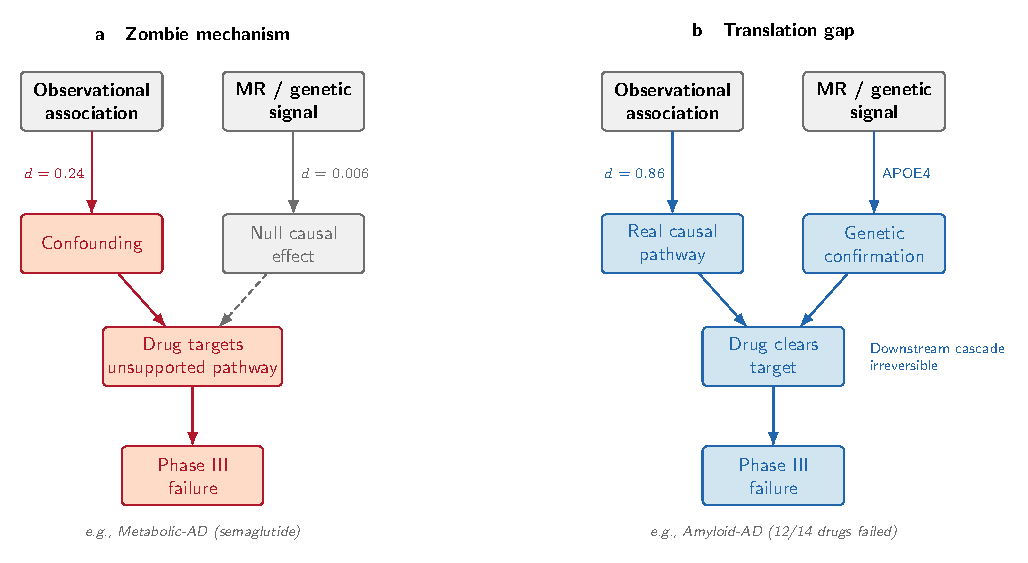
\includegraphics[width=\textwidth]{figures/fig2_failure_modes.pdf}
\caption{\textbf{Two structurally distinct failure modes.}
\textbf{a},~Zombie mechanisms: the observational association ($d = 0.24$
for Metabolic-AD) reflects confounding; the MR/genetic signal is null
($d = 0.006$). Drugs target a phantom pathway and fail Phase~III.
\textbf{b},~Translation-gap mechanisms: both observational and genetic
evidence confirm the pathway is real (Amyloid-AD, APOE4 OR~$= 3.46$),
but the downstream neurodegenerative cascade is irreversible by the time
of intervention. Twelve of fourteen amyloid-targeting drugs failed.}
\label{fig:failure_modes}
\end{figure}

\subsection{Cross-domain boundary test}
\label{sec:boundary}

Applied to a psychiatric dataset (31 drugs, 24 classifiable from 6 disorder-level families), the classification dropped to 58\% accuracy with zero specificity. Depression and Schizophrenia, each containing 8--9 distinct mechanism classes, are both classified as discordant, predicting failure for all drugs---missing all 10 approvals.

The framework requires mechanism-level families. In neuroepidemiology, families map to specific biological pathways (amyloid clearance, B-cell depletion, metabolic signaling). In psychiatry, families map to diagnostic categories containing heterogeneous mechanisms. Disorder-level discordance reflects mechanistic heterogeneity within the diagnostic category, not a property of any individual drug target.

\subsection{The investigation paradox}

Families studied with more evidence types showed more cross-type disagreement, not less. Each evidence type operates at a different biological scale, captures different confounders, and measures different aspects of a complex causal process. Apparent consensus within one evidence type is not validation. A mechanism tested only with observational studies looks ``consistent'' by default.

\subsection{Cross-domain generalization: cardiometabolic mechanisms}
\label{sec:cardio}

The psychiatric boundary test (\S\ref{sec:boundary}) showed the method fails when families are defined at the diagnostic level. A stronger test asks: does it replicate in a disease domain where mechanism-level families are well-defined and ground truth is unambiguous? Cardiometabolic disease provides this test. MR is most mature in cardiology, trial outcomes are clear, and several textbook ``zombie'' mechanisms have been documented independently of our framework.

We applied the same deterministic classification (Algorithm~\ref{alg:discordance}) to ten cardiometabolic mechanism families (Table~\ref{tab:cardio}). Effect sizes were drawn from published MR studies and meta-analyses; the decision rule, the $|d| = 0.10$ threshold, and the pooling procedure were frozen from the neuroepidemiology analysis. No parameters were re-estimated. The cardiometabolic families were defined at the mechanism level (e.g., ``HDL/CETP'' rather than ``lipids''), matching the granularity used in neuroepidemiology; the family definitions themselves are a degree of freedom, and we discuss this in the Limitations.

This analysis is a validation test, not a discovery. The cardiometabolic zombie mechanisms (HDL, niacin, homocysteine, CRP, uric acid) are well-established in the MR literature, and their identification here recovers known results using our deterministic rule. The value is that the same frozen procedure, designed for neuroepidemiology, transfers without modification to a domain where ground truth is unambiguous.

\begin{table}[t]
\centering
\caption{Cardiometabolic mechanism families. OBS OR is from prospective observational meta-analyses; MR OR is from the cited Mendelian randomization study (units vary by family; see footnotes). MR status indicates whether the MR confidence interval excludes the null. Seven of eight families with known trial outcomes are correctly classified; uric acid is ambiguous (see text).}
\label{tab:cardio}
\small
\begin{tabular}{llllllc}
\toprule
Family & OBS OR & MR OR (95\% CI) & MR & Trial & Class & Correct? \\
\midrule
HDL / CETP$^\text{a}$ & 0.62 & 0.93 (0.68--1.26) & Null & Failed & Qual.\ disc. & \checkmark \\
Niacin / HDL$^\text{a}$ & 0.62 & 0.93 (0.68--1.26) & Null & Failed & Qual.\ disc. & \checkmark \\
Homocysteine$^\text{b}$ & 1.32 & 1.02 (0.98--1.07) & Null & Failed & Qual.\ disc. & \checkmark \\
CRP$^\text{c}$ & 1.37 & 1.00 (0.97--1.02) & Null & No benefit & Qual.\ disc. & \checkmark \\
Uric acid$^\text{d}$ & 1.07 & 1.05 (0.92--1.20) & Null$^*$ & Failed & Ambig. & ($\sim$) \\
\midrule
LDL / PCSK9$^\text{e}$ & 1.52 & 1.78 (1.58--2.01) & Causal & Approved & Concordant & \checkmark \\
Blood pressure$^\text{f}$ & 1.41 & 1.44 (1.35--1.55) & Causal & Approved & Concordant & \checkmark \\
Triglycerides$^\text{e}$ & 1.72 & 1.62 (1.24--2.11) & Causal & Approved & Concordant & \checkmark \\
\midrule
Lp(a)$^\text{g}$ & 1.13 & 0.94 (0.93--0.95) & Causal & \emph{Pending} & Concordant & --- \\
IL-6R$^\text{h}$ & 1.25 & 0.95 (0.93--0.97) & Causal & \emph{Pending} & Concordant & --- \\
\bottomrule
\end{tabular}

\vspace{1mm}
{\footnotesize
$^\text{a}$Per 1 SD HDL-C \citep{voight2012}. Niacin and CETP inhibitors share the same HDL-raising MR evidence.
$^\text{b}$OBS per 5 $\mu$mol/L; MR is MTHFR TT vs CC \citep{clarke2012}.
$^\text{c}$OBS per 1 SD log CRP (ERFC); MR per 20\% lower CRP \citep{elliott2009}.
$^\text{d}$Per 1 SD urate \citep{white2016}. $^*$Egger MR (pleiotropy-robust) is null; conventional MR is borderline significant (1.18, 1.08--1.29). OBS association is weak ($d = 0.04$). See text.
$^\text{e}$Per 1 mmol/L. LDL OBS from prospective meta-analyses \citep{ference2019ldl}; LDL MR from \citet{holmes2015}. TG OBS from Sarwar 2007 (top vs.\ bottom tertile); TG MR from \citet{holmes2015} unrestricted score.
$^\text{f}$Per 10 mmHg SBP for stroke; OBS from Lewington 2002 (PSC); MR from \citet{georgakis2020}.
$^\text{g}$OBS per 1 SD (ERFC); MR per 10 mg/dL lower \citep{burgess2018lpa}.
$^\text{h}$OBS per 1 SD log IL-6 (ERFC); MR per allele \citep{interleukin2012}.
}
\end{table}

Four zombie mechanisms---HDL/CETP, niacin/HDL, homocysteine/B-vitamins, and CRP---each have moderate-to-strong observational associations with cardiovascular risk and null MR causal estimates (CI includes 1). All four produced drug failures: torcetrapib, dalcetrapib, and evacetrapib (CETP inhibitors); AIM-HIGH and HPS2-THRIVE (niacin); B-vitamin supplementation trials; and canakinumab's null primary endpoint in CANTOS despite reducing CRP. Note that niacin/HDL and HDL/CETP share the same underlying MR evidence \citep{voight2012}; they appear as separate families because the drug classes differ, but the genetic evidence is not independent.

Uric acid is ambiguous. The observational association is weak (OR 1.07 per 1 SD), and the MR evidence depends on method: conventional MR suggests a causal effect (OR 1.18, 95\% CI 1.08--1.29) while Egger MR, which accounts for pleiotropic instruments, does not (OR 1.05, 95\% CI 0.92--1.20; \citealp{white2016}). The allopurinol trial (ALL-HEART) found no cardiovascular benefit. Under our framework, the weak observational association ($d = 0.04$) and null Egger MR ($d = 0.03$) yield concordance at a near-null level---the evidence agrees that uric acid has little causal relevance for CHD. The concordance-to-approve mapping produces the wrong prediction; a ``null concordance'' rule (both types negligible $\to$ no target $\to$ predict failure) would handle this case correctly.

Three true positives---LDL/PCSK9, blood pressure, and triglycerides---have causal MR signals (CIs excluding 1) and approved drug classes.

Combined with the neuroepidemiology results (7/8 scored families correct, with BMI~$\to$~MS excluded as prediction pending), the method correctly classifies 7/7 unambiguous cardiometabolic families. Across both domains, 14 of 15 unambiguous family-level outcomes are correctly classified (permutation $p = 0.001$; see pre-registration for power analysis and false positive rate verification). The sole miss is vitamin~D supplementation. The classification rule and threshold are identical across domains.

\paragraph{Prospective predictions.}
Two cardiometabolic families have causal MR signals and Phase~III trials approaching readout. Lp(a)-lowering (pelacarsen, an antisense oligonucleotide targeting hepatic Lp(a) synthesis; concordant etiologic evidence) and IL-6 pathway inhibition (ziltivekimab, a monoclonal antibody targeting the IL-6 ligand; concordant etiologic evidence) are classified as ``Approve'' by the frozen rule. A caveat: the MR instrument for IL-6R uses variants in \emph{IL6R}, while ziltivekimab targets the IL-6 ligand rather than the receptor---the instrument and drug act on the same pathway but at different nodes. These predictions were registered before trial readout \textcolor{red}{[PREREG: commit SHA and date to be inserted]}.

\section{Discussion}

\subsection{Filling the GRADE gap}

GRADE's five dimensions operate within a single study design. Cross-type $Q$ adds a sixth: does the evidence hold up across designs? When MR finds no causal pathway (OR~1.01 for T2D-AD) while observational evidence shows a moderate association (RR~1.53), that discrepancy contains information GRADE cannot capture. The direction of the discrepancy diagnoses confounding.

Triangulation \citep{lawlor2016} captures the right intuition---multiple evidence types with different biases should converge on a true effect---but provides no quantitative test. Our contribution is complementary rather than competing: triangulation is about \emph{convergence} boosting credibility; cross-type $Q$ is about \emph{divergence} diagnosing failure mode. Convergence is the default expectation; what is informative is when and how evidence types diverge.

\subsection{Etiologic evidence as a screening tool}

The two-stage analysis points toward a practical screening role for etiologic $Q$ in drug development. Before committing to Phase~III for a novel target:

\begin{enumerate}
\item Compute Cochran's $Q$ across etiologic evidence types for the target mechanism.
\item If the MR/genetic causal signal is null while the observational association is positive $\to$ the mechanism is likely a zombie $\to$ high Phase~III failure risk.
\item If etiologic evidence is concordant $\to$ the mechanism is likely real $\to$ proceed, but concordance does not guarantee interventional success.
\end{enumerate}

This is a one-sided screen: a null MR signal is a strong negative indicator, but a positive MR signal is not a guarantee. The amyloid case demonstrates the asymmetry.

\subsection{Why etiologic concordance is necessary but insufficient}

The amyloid case illustrates a general principle. APOE4 is one of the strongest known genetic risk factors for any common disease (OR~3.46 per allele). Amyloid PET positivity robustly predicts AD conversion. The etiologic evidence is concordant. Drugs targeting amyloid clearance mostly fail.

The gap between etiologic concordance and interventional success reflects the difference between ``the mechanism is involved in pathogenesis'' and ``intervening on the mechanism at this stage reverses pathology.'' Amyloid accumulation may be an upstream causal factor in AD, but by the time clinical disease manifests, the downstream cascade (tau tangles, synaptic loss, neuroinflammation) may have become self-sustaining---though this mechanistic explanation remains a hypothesis rather than an established fact. The recent FDA approvals of lecanemab and donanemab via accelerated and traditional pathways remain controversial, with debate over whether statistically significant slowing on CDR-SB (27--35\%) constitutes clinical benefit. An estimated \$40 billion in failed trials \citep{cummings_zhong2014} targeted a mechanism that was etiologically valid but therapeutically insufficient.

The method performs more cleanly on MS than on AD. MS mechanism families map to specific biological pathways (B-cell depletion, vitamin~D, EBV) with relatively homogeneous drug targets within each family. AD families are more heterogeneous: ``amyloid'' encompasses production-pathway inhibitors, passive immunotherapy, and active immunotherapy, which may have distinct mechanisms of failure.

\section{Limitations}

The etiologic-only analysis classifies 8 of 38 holdout drugs---the remainder fall in families without multi-type etiologic evidence. The analysis is powered to demonstrate proof-of-concept (7/8 correct), not to establish population-level accuracy. The retrospective analysis including RCT evidence is circular for families whose RCT arm derives from holdout drugs---it should be interpreted as concordance, not prediction.

\paragraph{Threshold sensitivity.} The threshold $|d| = 0.10$ for qualitative versus quantitative discordance was chosen on substantive grounds (Cohen's negligible-effect boundary), not optimized. Anti-CD20-MS has GEN $d = 0.10$, sitting exactly on this boundary: at $d = 0.099$ the classification flips from quantitative discordance (approve) to qualitative discordance (fail), misclassifying four approved drugs. At thresholds of $d = 0.08$ and $d = 0.12$, the neuro classification is unchanged (7/8 correct at both). The result is robust to small perturbations but depends on the Anti-CD20 boundary case.

\paragraph{Family granularity.} Mechanism families are defined at the biological-pathway level, but the granularity is not uniquely determined. Semaglutide (assigned to Metabolic-AD) is a GLP-1 agonist with both metabolic and direct neuroprotective effects; the family assignment assumes the metabolic pathway is the relevant one. In the cardiometabolic domain, ``HDL/CETP'' could be split into genetic HDL-raising (null for CHD) and pharmacological CETP inhibition (which also raises LDL and has off-target toxicity). The family definitions are a degree of freedom, and different choices could change classifications.

\paragraph{Instrument-target alignment.} MR instruments are proxies for drug mechanisms, not direct models. The FCRL3 instrument for Anti-CD20-MS captures B-cell biology but not the ADCC mechanism of ocrelizumab; the IL6R instrument for IL-6 pathway inhibition targets the receptor while ziltivekimab targets the ligand. These mismatches do not invalidate the etiologic signal (both concern the same biological pathway) but they weaken the correspondence between MR evidence and drug mechanism.

Prospective validation---pre-registering etiologic classifications for mechanisms entering Phase~III and evaluating at trial readout---is the definitive test.

\section{Conclusion}

Three contributions emerge from this analysis. First, etiologic evidence discordance (observational versus MR/genetic) correctly classifies drug outcomes for the families it can assess---zombie mechanisms with null MR signals produce drug failures. Second, etiologic concordance is necessary but insufficient for drug success---the amyloid case shows that a mechanism can be etiologically valid and therapeutically insufficient. Third, these two failure modes are structurally different and demand different responses: zombies should be retired from target pipelines; translation-gap mechanisms need different therapeutic strategies, not abandonment of the mechanism.

The practical recommendation: compute Cochran's $Q$ across etiologic evidence types before committing to Phase~III. A null MR signal for the target mechanism is a strong negative indicator. A positive MR signal is necessary but insufficient.

\bibliographystyle{plainnat}
\bibliography{references}

\end{document}
